\documentclass[aps,pra,showpacs]{revtex4}




% this is the preamble created by tikzit, we can edit this in the final document to change the shapes we use for nodes, edge styles, etc... 
% just be sure to use the same name for the same kind of node/edge in any figures you make

\usepackage[svgnames]{xcolor}
\usepackage{tikz}
\usetikzlibrary{decorations.markings}
\usetikzlibrary{shapes.geometric}
%\pagestyle{empty}

\pgfdeclarelayer{edgelayer}
\pgfdeclarelayer{nodelayer}
\pgfsetlayers{edgelayer,nodelayer,main}

\tikzstyle{none}=[inner sep=0pt]

\tikzstyle{rn}=[circle,fill=Red,draw=Black,line width=0.8 pt]
\tikzstyle{gn}=[circle,fill=Lime,draw=Black,line width=0.8 pt]
\tikzstyle{yn}=[circle,fill=Yellow,draw=Black,line width=0.8 pt]
\tikzstyle{auxiliary_qubit}=[circle,fill=Red,draw=Black,scale=0.8]
\tikzstyle{logical_qubit}=[circle,fill=Black,draw=Black,scale=0.8]
\tikzstyle{emb_logical_qubit}=[circle,fill=Gray,draw=Black,scale=0.8,line width=2.000]
\tikzstyle{emb_auxiliary_qubit}=[circle,fill=Red,draw=Black,scale=0.8,line width=2.000]
\tikzstyle{unused_qubit}=[circle,fill=Gray,draw=Gray,scale=0.8]
\tikzstyle{arrow_end}=[circle,fill=none,draw=none,scale=.1]




\tikzstyle{simple}=[-,draw=Black,line width=1.000]
\tikzstyle{added}=[-,draw=green,line width=1.000]
\tikzstyle{unused}=[-,draw=gray,line width=0.500]
%\definecolor{tempcolor}{rgb}{.7,.9,.7}
%\tikzstyle{unused_added}=[-,draw=tempcolor,line width=1.000]
%\tikzstyle{unused_added}=[-,draw=green,draw opacity=1,line width=1.000,dashed]
\tikzstyle{unused_added}=[-,draw=cyan,draw opacity=1,line width=0.5]
\tikzstyle{embedding}=[-,draw=Black,line width=3.000]
\tikzstyle{arrow}=[-,draw=Black,postaction={decorate},decoration={markings,mark=at position .5 with {\arrow{>}}},line width=2.000]


 % preamble which globally defines nodes and edges for tikz, edit this file to change nodes and edges


\newcommand{\rc}{\mathbf{\rho}}



\begin{document}



\begin{table}
\begin{centering}
\begin{tabular}{|c|c|c|}
\hline 
Symbol & Meaning & file  \tabularnewline
\hline 
\hline 
\input{visual_elements_for_table/simple_edge.tikz}& Interaction between qubits (not-minor embedding) & visual\_elements\_for\_table/simple\_edge.tikz \tabularnewline
\hline 
\input{visual_elements_for_table/added.tikz}& Interaction which is added in Pegasus and not in Chimera (used) & visual\_elements\_for\_table/added.tikz \tabularnewline
\hline 
\begin{tikzpicture}
	\begin{pgfonlayer}{nodelayer}
		\node [style={arrow_end}] (0) at (-1, -0) {};
		\node [style={arrow_end}] (1) at (0, -0) {};
		\node [style={arrow_end}] (2) at (0, -0) {};
	\end{pgfonlayer}
	\begin{pgfonlayer}{edgelayer}
		\draw [style=unused] (0) to (1);
	\end{pgfonlayer}
\end{tikzpicture}
& Interaction which is present in chimera but not used & visual\_elements\_for\_table/unused.tikz \tabularnewline
\hline 
\input{visual_elements_for_table/unused_added.tikz}& Interaction which is added in Pegasus and not in Chimera (not used) & visual\_elements\_for\_table/unused\_added.tikz \tabularnewline
\hline 
\input{visual_elements_for_table/embedding.tikz}& Interaction which is used for minor embedding & visual\_elements\_for\_table/embedding.tikz \tabularnewline
\hline 

\begin{tikzpicture}
	\begin{pgfonlayer}{nodelayer}
		\node [style=logical_qubit] (0) at (0, -0) {};
	\end{pgfonlayer}
\end{tikzpicture}
& Logical qubit, not part of minor embedding & visual\_elements\_for\_table/logical\_qubit.tikz \tabularnewline
\hline 
\input{visual_elements_for_table/emb_logical_qubit.tikz}& Logical qubit, part of minor embedding & visual\_elements\_for\_table/emb\_logical\_qubit.tikz \tabularnewline
\hline 

\begin{tikzpicture}
	\begin{pgfonlayer}{nodelayer}
		\node [style=emb_auxiliary_qubit] (0) at (0, -0) {};
	\end{pgfonlayer}
\end{tikzpicture}
& Logical qubit, part of minor embedding & visual\_elements\_for\_table/emb\_auxiliary\_qubit.tikz \tabularnewline
\hline 
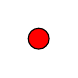
\begin{tikzpicture}
	\begin{pgfonlayer}{nodelayer}
		\node [style=auxiliary_qubit] (0) at (0, -0) {};
	\end{pgfonlayer}
\end{tikzpicture}
& Auxiliary qubit & visual\_elements\_for\_table/auxiliary\_qubit.tikz \tabularnewline
\hline 
\input{visual_elements_for_table/unused_qubit.tikz}& Unused qubit & visual\_elements\_for\_table/unused\_qubit.tikz \tabularnewline

\hline 
\end{tabular}
\par\end{centering}

\caption{Table defining visual elements used in figures and giving filenames for single visual elements}


\end{table}



\end{document}
